\chapter{VALIDACIÓN DE LA INFORMACIÓN CON ESTACIONES ACTIVAS}


Actualmente en el departamento de Nariño se han instalado alrededor de 25 estaciones con la capacidad de reportar datos radiación solar, viento, 
precipitación, temperatura y humedad del aire Figura~\ref{fig:stationsalternar}; de las 25 estaciones instaladas se realizó la selección de 11 
estaciones Figura~\ref{fig:stationstested}, esta decisión fué aplicada por inconvenientes en las estaciones como tiempos cortos de reporte de estaciones, debido 
a que muchas estaciones fueron instaladas a finales del año 2015, este corto tiempo de reporte no permite medir con gran certeza la relación entre 
la serie de tiempo construida y los reportes de las estaciones que fueron instaladas hace pocos meses, otros factores que provocaron que se descartaran varias 
estaciones son los errores en el reporte de datos ocasionados por fallas en la calibración de los dispositivos, interrupciones en reporte 
de información, diferencia en tipo de dispositivo y factores exógenos que inciden de forma importante en el reporte de datos. 
\begin{figure}[htb]
  \centering 
  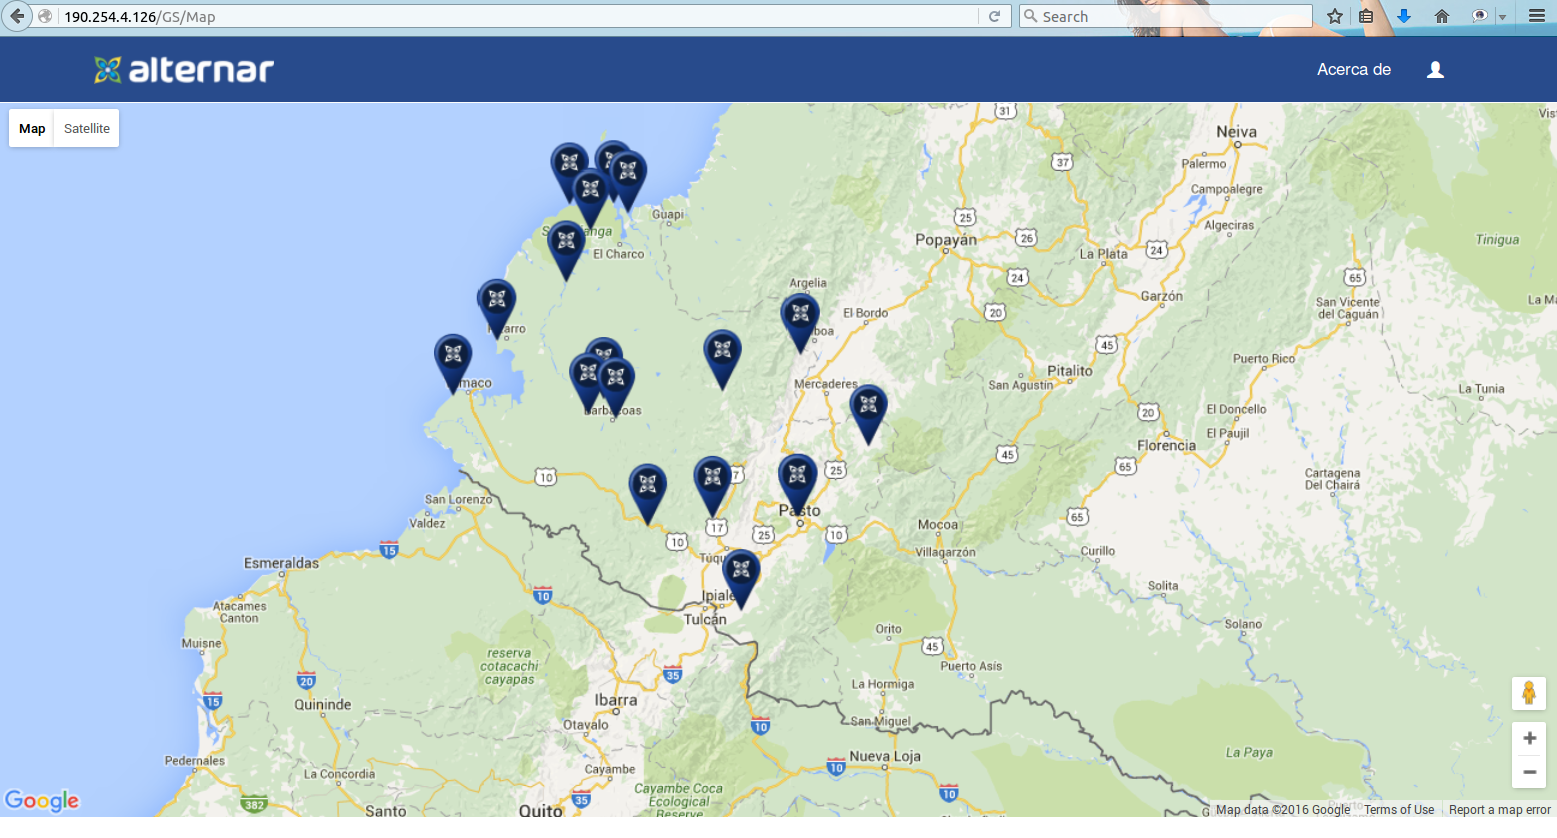
\includegraphics[scale=0.27]{pictures/stationsalternar.png}
  \caption{Plataforma de reporte y ubicación de estaciones del proyecto Alternar}
  \label{fig:stationsalternar}
\end{figure}
\begin{figure}[htb]
  \centering 
  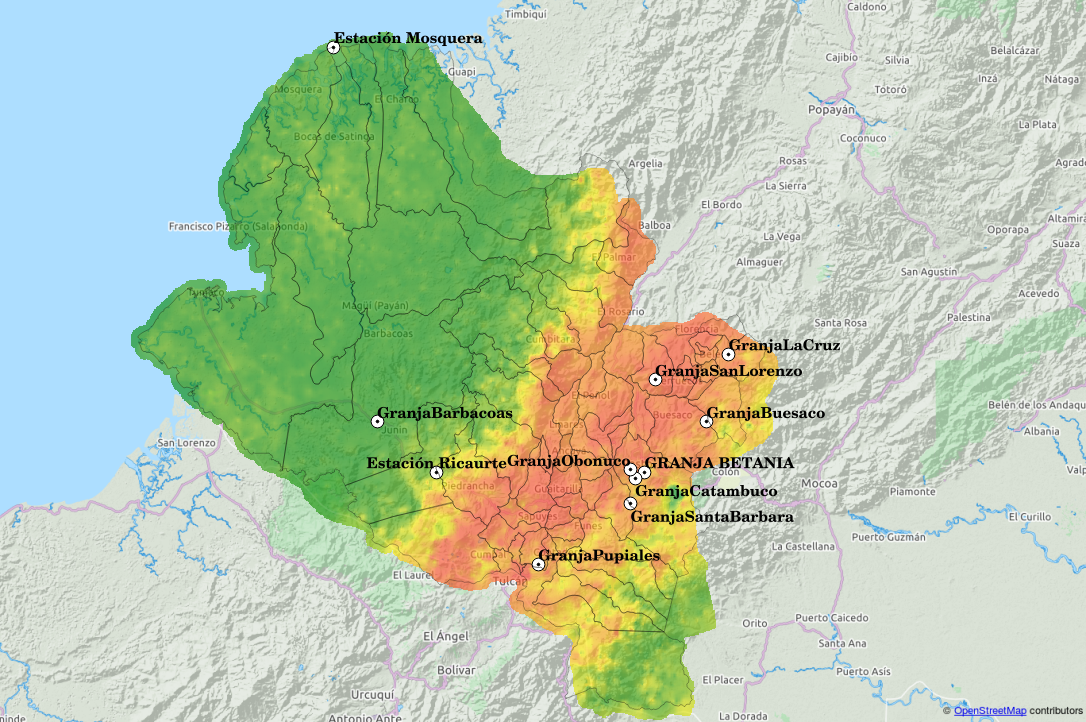
\includegraphics[scale=0.45]{pictures/stationstested.png}
  \caption{Estaciones seleccionadas para proceder a validación de datos de radiación solar}
  \label{fig:stationstested}
\end{figure}
En la validación es necesario gran cantidad de muestras que permitan establecer una mayor certeza en el análisis de los datos reales con los datos de las imágenes
satelitales, por este motivo es importante destacar que las imágenes satelitales MODIS tienen una resolución temporal diaria mientras que las imágenes 
satelitales LandSat tiene una resolución temporal cada 16 dias, por este motivo se descartó para la validación los datos de LandSat.

Al disponer del registro histórico de las 11 estaciones, se procede a realizar la validación de los datos de radiación solar; para el proceso de validación es 
necesario obtener los promedios mensuales de las 11 estaciones y los promedios mensuales de radiación de la serie de tiempo construida ubicando la zona 
correspondiente, los promedios obtenidos permiten establecer una correlación buena entre los datos de radiación solar de las estaciones y los datos de radiación 
solar de MODIS. A continuación se puede observar los resultados obtenidos del análisis realizado a las 11 estaciones con reportes superiores a 5 meses y 
la serie de tiempo de radiación solar obtenida del sensor MODIS.

\begin{table}[H]
\centering
\begin{tabular}{ >{\arraybackslash}m{7cm} >{\centering\arraybackslash}m{5cm} >{\centering\arraybackslash}m{3cm}}
\hline
Estación & Ubicación & $R^2$ \\
\hline \hline
Estación Mosquera& (-78.333333,2.655) & 86,57 \% \\
\hline
Estación Ricaurte & (-77.975833,1.186944) & 90,33 \%\\
\hline
Granja Barbacoas & (-78.18173,1.361483333) & 74,09 \%\\
\hline
Granja Betania & (-77.257028,1.186317) & 84,64 \%\\
\hline
Granja Buesaco & (-77.04079,1.35932) & 76,55 \%\\
\hline
Granja Catambuco & (-77.290397,1.166761) & 60,82 \%\\
\hline
Granja La Cruz & (-76.9640701,1.5955594) & 91,26 \%\\
\hline
Granja Obonuco & (-77.305556,1.193458) & 71,52 \%\\
\hline
Granja Pupiales & (-77.624667,0.867483) & 90,47 \%\\
\hline
Granja San Lorenzo & (-77.219125,1.503858) & 65,11 \%\\
\hline
Granja Santa Barbara & (-77.305544,1.078422) & 81,27 \%\\
\hline
\end{tabular}
\caption{Análisis datos de radiación solar Reporte Estaciones Vs Serie de Tiempo MODIS.}
\label{tabla:validacion}
\end{table}